\section{業務の流れ}

本システムは、小規模から中規模のゲーム大会において、大会情報、競技者情報、対戦情報および試合結果
を一元管理し、大会主催者の運営負担を軽減するとともに、競技者と観戦者に必要な情報を提供する Web 
システムである。

主催者は大会名、対象ゲーム、開催日時、開催場所、参加条件および大会形式などを登録し、大会を公開す
る。競技者は Web ブラウザから大会を検索し、氏名、プレイヤー名、メールアドレスなどを入力して参加
登録を行う。入力内容は Web システムで確認され、問題がなければデータベースに保存される。 

主催者は競技者一覧を確認し、受付状況を管理する。大会開催時には、競技者情報と大会形式に基づいてト
ーナメント表を作成する。試合終了後は競技者または主催者が試合結果を登録し、確認された結果をデータ
ベースに保存する。シングルエリミネーションでは勝者を次のラウンドへ反映し、総当たり方式では勝利数
などを集計して順位を更新する。

観戦者は大会ページから大会全体の進行状況、トーナメント表、試合結果およびライブ配信のURLを確認で
きる。また、特定の選手を検索・お気に入り登録し、その選手の過去の試合結果、現在の試合状況、次の対
戦相手およびトーナメント上の位置を確認できる。

\subsection{業務の基本的な流れ} 
\begin{table}[H]
  \centering
  \caption{業務の基本的な流れ}
  \label{tab:hardware}
  \begin{tabularx}{\linewidth}{|l|l|l|X|}
    \hline
    \rowcolor{tableblue}
    \multicolumn{1}{|c|}{順序} & \multicolumn{1}{c|}{担当} & \multicolumn{1}{c|}{業務内容} & \multicolumn{1}{c|}{システムの処理} \\ \hline
    1 & 主催者  & 大会情報の登録  & 大会情報を受け取り、データベースに保存して公開する。 \\ \hline
    2 & 競技者 & 大会への参加登録 & 入力内容・形式・重複を確認し、競技者と参加情報を保存する。 \\ \hline
    3 & 主催者  & 競技者の確認・受付 & 競技者一覧を表示し、受付済み／未受付を管理する。 \\ \hline
    4 & 主催者 & トーナメント作成 & 登録競技者と大会形式に基づき対戦組み合わせを作成する。 \\ \hline
    5 & 主催者/競技者 & 試合結果の登録・確認 & 結果を確認して確定し、試合情報と大会進行状況を更新する。 \\ \hline
    6 & 主催者/観戦者 & 大会情報の閲覧 & 対戦相手、試合予定、結果、注目選手情報などを表示する。 \\ \hline
  \end{tabularx}
\end{table}

\begin{figure}[H]
    \centering
    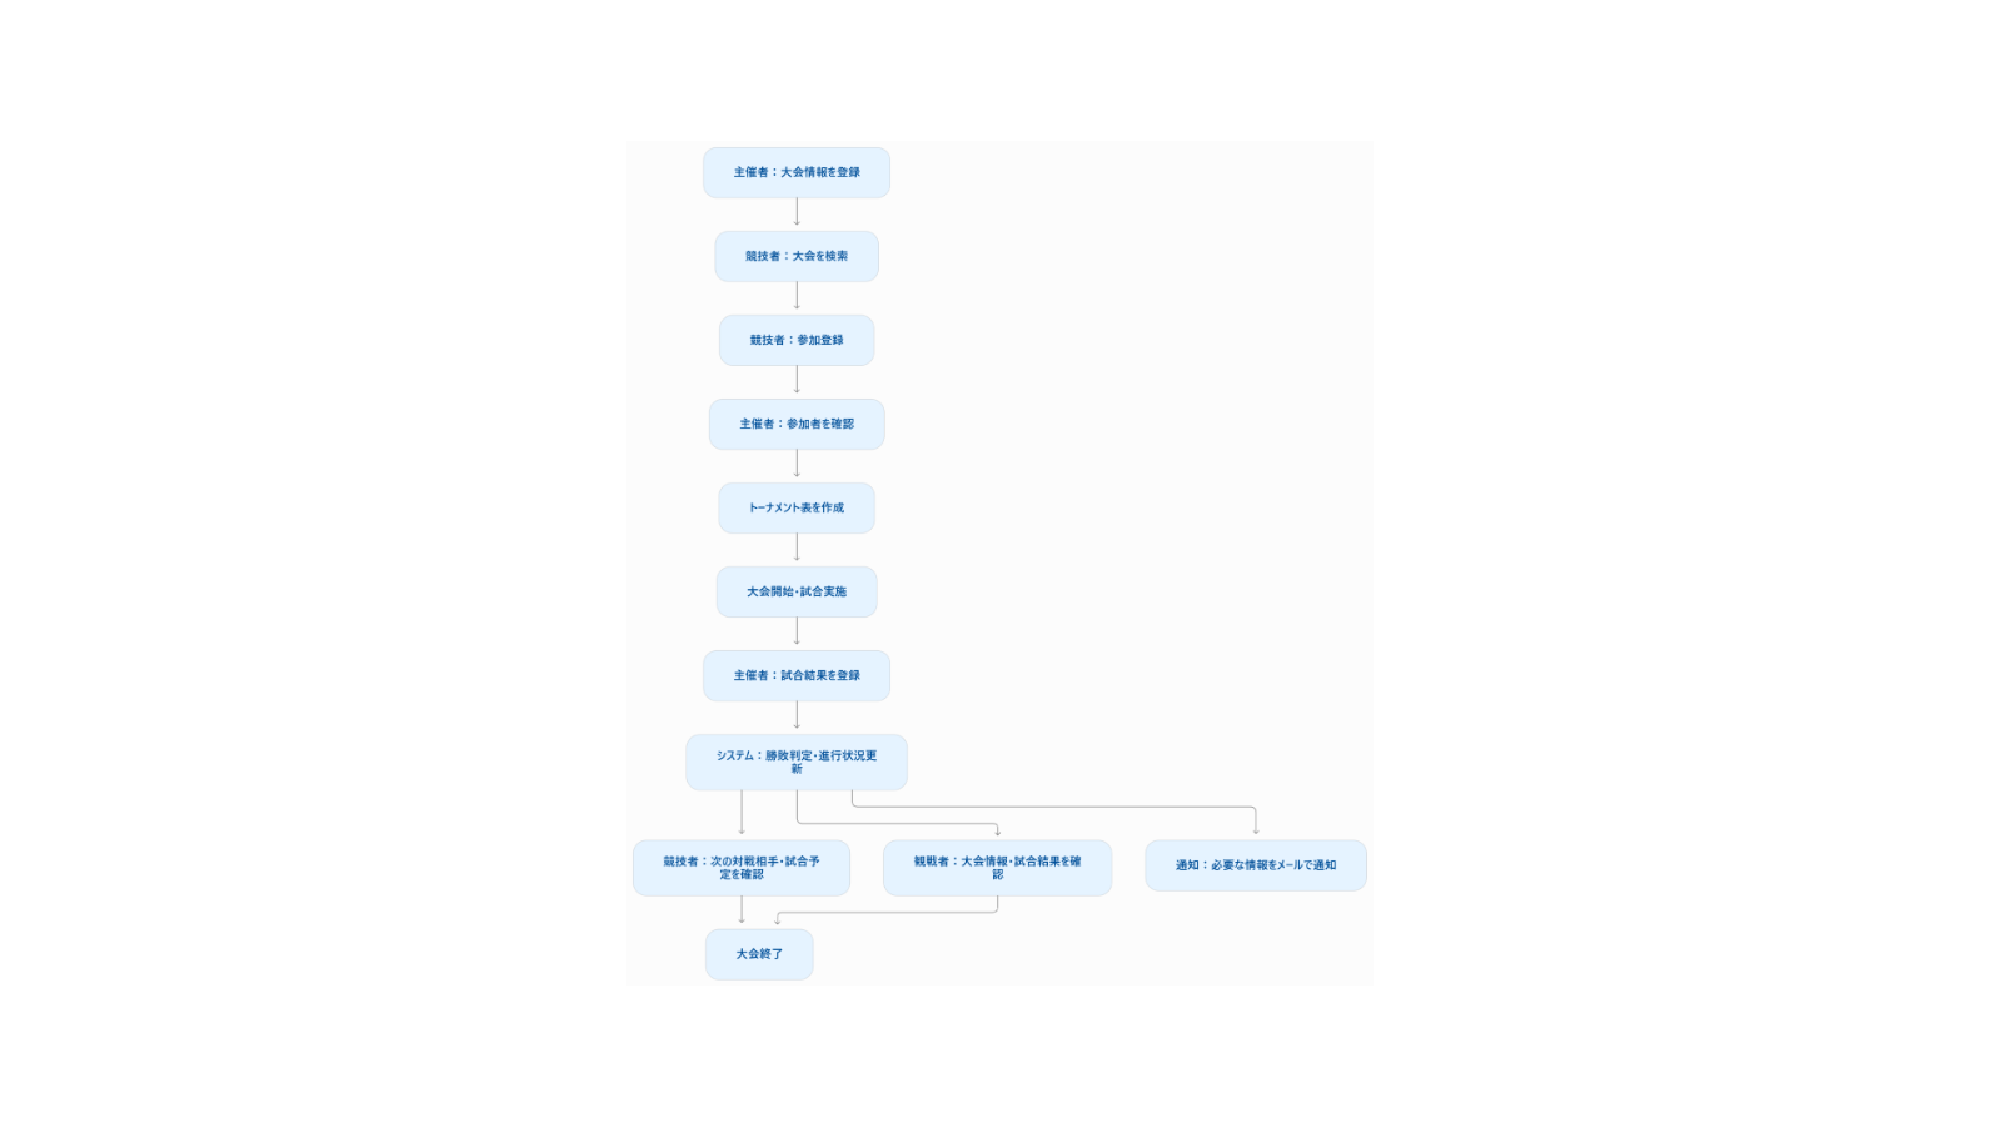
\includegraphics[width=\linewidth]{figures/02/business_flow.pdf}
    \caption{業務の基本的な流れ}
    \label{fig:business_flow}
\end{figure}